%%%%%%%% ICML 2020 EXAMPLE LATEX SUBMISSION FILE %%%%%%%%%%%%%%%%%

\documentclass{article}

% Recommended, but optional, packages for figures and better typesetting:
\usepackage{microtype}
\usepackage{graphicx}
\usepackage{subfigure}
\usepackage{booktabs} % for professional tables

% hyperref makes hyperlinks in the resulting PDF.
% If your build breaks (sometimes temporarily if a hyperlink spans a page)
% please comment out the following usepackage line and replace
% \usepackage{icml2020} with \usepackage[nohyperref]{icml2020} above.
\usepackage{hyperref}

% Attempt to make hyperref and algorithmic work together better:
\newcommand{\theHalgorithm}{\arabic{algorithm}}

% Use the following line for the initial blind version submitted for review:
\usepackage{icml2020}

% If accepted, instead use the following line for the camera-ready submission:
%\usepackage[accepted]{icml2020}

% Packages I added:
\usepackage{todo}
% \presetkeys%
%     {todonotes}%
%     {inline,backgroundcolor=yellow}{}
\usepackage{amsmath}
\usepackage{amsthm}

\newtheorem{defn}{Definition}

% The \icmltitle you define below is probably too long as a header.
% Therefore, a short form for the running title is supplied here:
\icmltitlerunning{Deep MR}

\begin{document}

\twocolumn[
\icmltitle{Deep Mendelian Randomization: Using Mendelian Randomization to Detect Learned Causal Relationships in Deep Learning Models}

% It is OKAY to include author information, even for blind
% submissions: the style file will automatically remove it for you
% unless you've provided the [accepted] option to the icml2020
% package.

% List of affiliations: The first argument should be a (short)
% identifier you will use later to specify author affiliations
% Academic affiliations should list Department, University, City, Region, Country
% Industry affiliations should list Company, City, Region, Country

% You can specify symbols, otherwise they are numbered in order.
% Ideally, you should not use this facility. Affiliations will be numbered
% in order of appearance and this is the preferred way.
\icmlsetsymbol{equal}{*}

\begin{icmlauthorlist}
\icmlauthor{Stephen Malina}{equal,cu}
\icmlauthor{David Knowles}{equal,cu,nygc}
\end{icmlauthorlist}
\icmlcorrespondingauthor{Stephen Malina}{sdm2181@columbia.edu}

\icmlaffiliation{to}{Department of Computer Science, Columbia University, New York, NY}
\icmlaffiliation{nygc}{New York Genome Center, New York, NY}

% You may provide any keywords that you
% find helpful for describing your paper; these are used to populate
% the "keywords" metadata in the PDF but will not be shown in the document
\icmlkeywords{Mendelian Randomization, Deep Learning, Causal Inference}

\vskip 0.3in
]

% this must go after the closing bracket ] following \twocolumn[ ...

% This command actually creates the footnote in the first column
% listing the affiliations and the copyright notice.
% The command takes one argument, which is text to display at the start of the footnote.
% The \icmlEqualContribution command is standard text for equal contribution.
% Remove it (just {}) if you do not need this facility.

%\printAffiliationsAndNotice{}  % leave blank if no need to mention equal contribution
\printAffiliationsAndNotice{\icmlEqualContribution} % otherwise use the standard text.

\begin{abstract}
\end{abstract}

\section{Introduction}
\label{introduction}
Recently, deep learning models have been used to classify genomic features such as transcription factor binding \cite{alipanahi2015predicting, zhou2015predicting}, chromatin accessibility \cite{zhou2015predicting, kelley2016basset}, the presence / absence of histone marks \cite{yin2019deephistone}, and RNA binding protein binding \cite{alipanahi2015predicting, pan2017rna, gandhi2018cdeepbind, zheng2018deep}. These models achieve high predictive accuracy on these tasks and recognize features that match those found in experiments. Furthermore, multi-task models such as DeepSEA~\cite{zhou2015predicting} achieve high accuracy simultaneously on multiple genomic feature prediction tasks. Given this, we would like to understand whether these multi-task models, through learning to predict multiple features jointly, gain an understanding of the causal relationships between these features.

That said, answering this question requires a methodology that can identify causal relationships in the presence of potential unobserved confounding between cause and effect. To that end, we employ Mendelian randomization \cite{lawlor2008mendelian}, an instrumental variable approach for causal inference, to estimate learned causal effects in genomic deep learning models. Our algorithm obtains local (sequence level) and global (genome level) estimates of the linear causal relationship between two biological processes learned by a multi-task genomic prediction model. In this work, we apply our approach to estimating the learned causal effect of transcription factor binding on chromatin accessibility in a single cell type, but our method can in principle be applied to other processes that are believed to satisfy the instrumental variable assumptions.

\section{Related Work}
\subsection{Deep Learning Model Interpretability}
Local interpretability methods such as saliency maps \cite{simonyan2013deep}, guided back-propagation \cite{springenberg2014striving}, DeepLift \cite{shrikumar2017learning}, and Deep SHAP \cite{lundberg2017unified}, characterize how specific input features influence deep learning model predictions and, in some cases, intermediate layer activations. Even DeepLift, which was designed with genomic deep learning in mind, focus on interpreting individual model predictions rather than discovering higher-level properties and therefore complement rather than compete with Deep MR.

Saturation in-silico mutagenesis characterizes how a model's predictions for an input change as a result of all possible point mutations to the input. Saturation mutagenesis has been used to assess the learned representations of genomic deep learning models such as DeepBind \cite{alipanahi2015predicting}, cDeepBind \cite{gandhi2018cdeepbind}, DeepSEA \cite{zhou2015predicting}, Basset \cite{kelley2016basset}, and others. In our work, we use saturation mutagenesis (combined with MC-dropout, see section \ref{sec:dl_uncertainty}) to generate a set of \textit{effect sizes} which we then provide as input to Mendelian randomization.

\subsection{Mendelian Randomization (MR)}
As alluded to above, Mendelian randomization is a technique for estimating linear causal effects in the presence of potential unobserved confounders. Mendelian randomization is a type of instrumental variable method in which the instrument(s) are genetic variants. While Mendelian randomization is typically used to estimate inter-phenotype causal effects from observational data, we use it in our work to estimate causal effects implied by model-generated data.

\begin{figure*}[htpb]
    \centering
    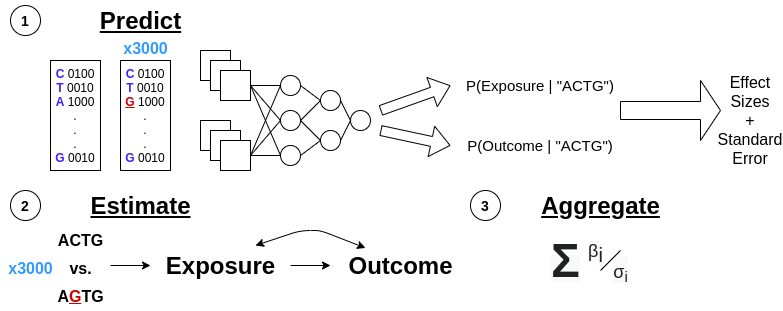
\includegraphics[width=.8\linewidth]{fig/model_overview.png}
    \caption{Graphical representation our algorithm's high-level steps. \underline{Predict} corresponds to steps 1 through 4 in section \ref{sec:algo_overview}. \underline{Estimate} corresponds to step 5 in section \ref{sec:algo_overview}. \underline{Aggregate} corresponds to step 6 in \ref{sec:algo_overview}.}
    \label{fig:model_overview}
\end{figure*}
\subsubsection{Mendelian Randomization Assumptions}
As depicted in figure \ref{fig:model_overview} under \underline{Estimate}, Mendelian randomization only produces valid causal effect estimates under the following assumptions\footnote{\citet{lawlor2008mendelian} provides a much more comprehensive overview of Mendelian randomization, its connection to instrumental variable methods, and their assumptions.}. Let $ Z $ be a variable we intend to use as an instrument (a genetic variant for example), $ X $ a purported cause (\textit{exposure}), and $ Y $ a purported effect (\textit{outcome}), and suppose that there may be unobserved confounding between $ X $ and $ Y $, denoted by $ U $. Then, Mendelian randomization's estimates are valid if:
\begin{enumerate}
    \item $ Z $ is independent of $ U $.
    \item $ Z $ is not independent of $ X $.
    \item $ Z $ only influences $ Y $ through $ X $.
\end{enumerate}

However, recent MR methods such as Robust Adjusted Profile Score \cite{zhao2018statistical}, MR-Egger \cite{bowden2015mendelian}, and the modal-based estimator \cite{burgess2018modal} seek to leverage multiple instruments to relax some of these assumptions without compromising the validity of results. In our work, we estimate causal effects using MR-Egger with the goal of being robust to weak instruments.

\subsection{Uncertainty Estimates from Deep Learning Models}
\label{sec:dl_uncertainty}
Since Mendelian randomization requires standard errors effect sizes, we need standard error estimates for our model predictions in addition to point predictions. In order to acquire them, we use Monte Carlo Dropout (MC-dropout) \citet{gal2016dropout}. MC-dropout is motivated by showing that a deep learning model can be thought of as a variational approximation to a Gaussian process. In practice, MC-dropout requires enabling dropout at test time, making repeated predictions for each sequence repeatedly (50 times in our case), and then computing predictive mean and variance as follows (assuming classification). 

Let $ X $ be a binary variable being predicted and $ S $ be our input. Denote the $ i $-th prediction for $ S $ with $ \hat{X}_i $ assuming $ i \in 1, \dots n $. Compute the predictive mean and variance as the sample mean and variance of the $ n $ predictions $ P(\hat{X}_i \mid S) $ for $ i \in 1, \dots, n $.

\section{Methods}
\begin{figure*}[ht]
    \centering
    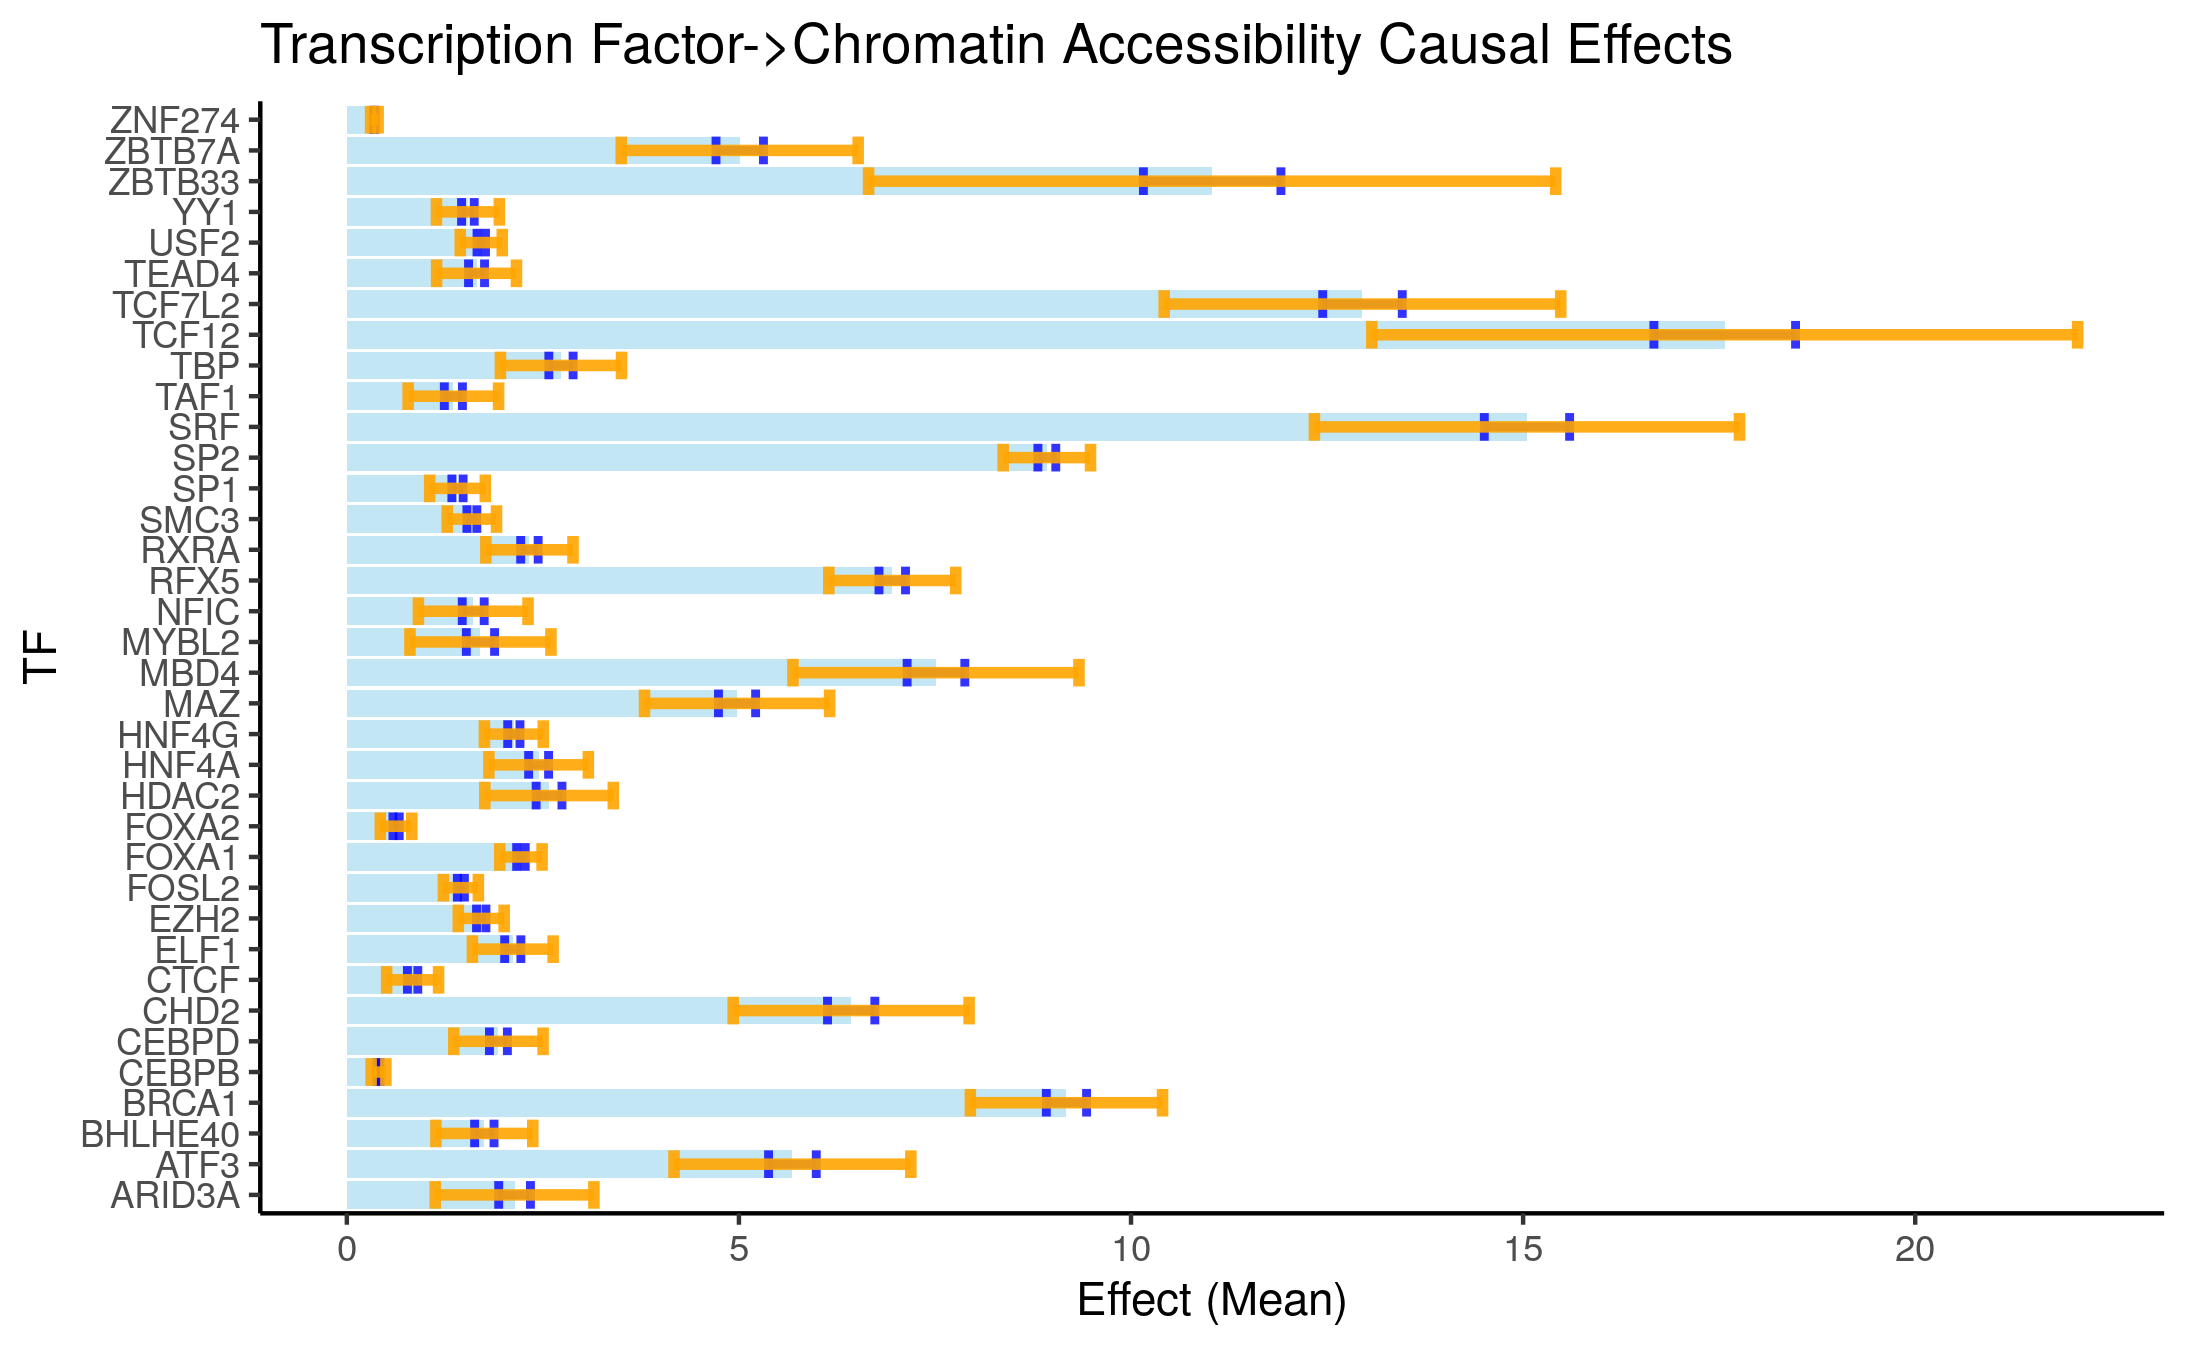
\includegraphics[width=0.8\linewidth]{fig/overall_ces.png}
    \caption{Per-transcription factor causaal effect estimates output by Deep MR's final step. The light blue bars show the magnitude of the overall causal effect estimated by the meta-analysis. Orange bars show \( \tau \)'s magnitude and dark blue the standard deviation of the mean's.}
    \label{fig:overall_ces}
\end{figure*}
\subsection{Algorithm Overview}
\label{sec:algo_overview}
Our algorithm attempts to estimate causal effect sizes between variables from predictions generated by a multi-task model. It requires as input a trained model\footnote{The model could in principle be a regression or classification model, but we focus on classification in our experiments and discussion.} and a set of one-hot encoded sequences, representing a sequence of nucleotides in our case, for the model to make predictions on. Following the MR literature, we refer to purported causes as \textit{exposures} and effects as \textit{outcomes}.

Given these inputs, our algorithm outputs a set of local, sequence-specific and exposure-specific causal effects and set of global, exposure-specific causal effects. It accomplishes this (see figure~\ref{fig:model_overview} for a visual depiction) via the following steps for each exposure:
\begin{enumerate}
    \item Randomly sample sequences to predict exposure and outcome values for (``reference sequences'').
    \item Perform \textit{saturation in-silico mutagenesis} for each reference sequence to generate \( \text{sequence\ length} \times \text{number\ of\ nucleotides} - 1 \) mutated sequences per original sequence.
    \item For each reference and set of mutated sequences, use MC-dropout \todo*{cite} to generate predictive means and standard errors of binding probabilities for the (reference|mutated) sequences.
    \item Generate \( (\text{sequence length} \times \text{alphabet size} - 1) \) \textit{effect sizes} by subtracting each reference sequence's predictive mean from the corresponding mutated sequences' predictive means. Also compute the standard errors of these differences.
    \item Estimate a per-exposure, per-sequence region causal effect by running Mendelian randomization on the per-exposure, per-sequence effect sizes and their standard errors.
    \item Estimate overall per-exposure factor causal effects using a meta-analysis.
\end{enumerate}

This leaves us with estimates of local (transcription factor and sequence level) and global (transcription factor level) causal effects. 

% \subsection{Exposure and Outcome Effect Size \& Standard Error Estimation}
% As part of the above, we need the predicted difference in both the exposure and outcome value for every mutated, reference sequence pair. Saturation mutagenesis and MC-dropout together provide us with predicted exposure and outcome differences for each mutated sequence, reference sequence pair, but only estimates for the standard errors of the individual predictions not the difference between the two. To obtain the latter quantity, the variance of the differences between the predicted exposure and outcome values for the mutated and reference sequences, we apply the following well-known identity
% \begin{equation}
%     \text{Var}(X - Y) = \text{Var}(X) + \text{Var}(Y) = 2 \cdot \text{Cov}(X, Y).
% \end{equation}
% This provides us with a standard error value which we give to Mendelian randomization along with our effect size estimates.

% \section{Overall Causal Effect Estimation}
% To estimate overall causal effects at the per-exposure level, we used an inverse-variance weighted random effects meta-analysis.

TODO: Question for David - should I include more here? I can talk about any of the sub-components (there's some commented out stuff in which I do that already). Or I can talk about some of the more subtle choices like only sampling sequences with binding, but that seems perhaps too in the weeds.


\section{Experimental Results}
\begin{figure*}[ht]
\centering
\begin{subfigure}
\centering
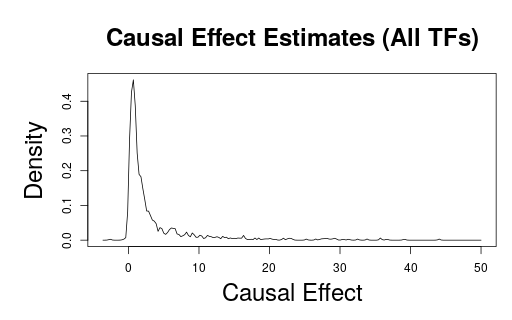
\includegraphics[width=.6\linewidth]{fig/all_tfs_ces_kde}
\end{subfigure}%
\begin{subfigure}
\centering
\includegraphics[width=.4\linewidth]{fig/FOXA1_ces_kde}
\label{fig:sub2}
\end{subfigure}
\begin{subfigure}
\centering
\includegraphics[width=.4\linewidth]{fig/EZH2_ces_kde}
\end{subfigure}
\caption{Kernel density estimate of causal effect estimates for all TFs (top), FOXA1 (middle), and EZH2 (bottom).}
\label{fig:ces_kdes}
\end{figure*}
To test our method, we used a pre-trained DeepSEA~\cite{zhou2015predicting} model provided by the Kipoi library~\cite{avsec2019kipoi} to estimate the learned causal effect of 36 transcription factors on chromatin accessibility in the HepG2 cell type. We drew our sequence regions from DeepSEA's held-out test set\footnote{Full list found in supplementary table 1 \hyperlink{https://www.nature.com/articles/nmeth.3547\#Sec12}{here}.}, which was generated via processing the results of ChIP-seq (for transcription factors) and DNase-seq (for chromatin accessibility) experiments as part of the ENCODE project\cite{encode2004encode}.

For each transcription factor, we randomly sampled 25 (1000 base pair) sequences on which binding was experimentally observed to occur and followed the process described above. 

\subsection*{Sequence-level causal effect estimates concentrate around 0}
As we'd expect given random sampling of sequences, the first graph in figure~\ref{fig:ces_kdes} shows that, across all transcription factors, the mode of causal effects is very close to 0. This gives us some confidence that, Mendelian randomization is able to correctly filter out noise when the set of mutation effects for mutated versions of a reference sequence show no underlying pattern. 

\subsection*{Causal effect estimates vary significantly across transcription factors}
The results of our final meta-analysis step, shown in figure \ref{fig:overall_ces}, imply significant variation in the strength of causal relationships between different transcription factors and chromatin accessibility. While all causal effects are positive, certain transcription factors' binding seems to have a very large positive influence on chromatin accessibility. We intend to try and understand the degree to which this reflects modeling assumptions and matches experimental evidence in future work.

% As evidenced by the number of large \( \tau^2 \) values in table \ref{fig:overall_ces}, we see significant variation in causal effect estimates for individual transcription factors.
\subsection*{Causal effect estimates vary significantly across sequences for individual transcription factors}
To try and better understand how our results relate to experimental evidence, we inspected the sequence-level causal effect estimates for a known transcriptional enhancer, FOXA1, and transcriptional repressor, EZH2, in the HepG2 cell type. Based purely on the coarse grained enhancer (FOXA1) and repressor (EZH2) (in the HepG2 cell type) classification, we'd expect FOXA1's causal effect estimates to be mostly positive and EZH2's estimates to be mostly negative. As figure \ref{fig:ces_kdes} shows, FOXA1's causal effects are all positive and all but one of EZH2's causal effect estimates are positive. While EZH2's results do not match our expectations, it's interesting that one of its effects is negative given that it's a known repressor. In future work, we hope to apply our method to sequences with known binding / accessibility relationships to determine whether the results match finer-grain patterns observed experimentally and understand whether the bias towards positive results is a model artifact or not.

TODO - Question for David: does this warrant more discussion? Would that belong here or in Discussion?
TODO - Question for David: Does it make sense to include any of the interpretation stuff we did in here? I feel like the results were more of a check for us but maybe the highlighted logos would be worth including regardless?

\section{Discussion}
In our experiment, Deep MR identifies a consistent positive effect of transcription factor binding on chromatin accessibility. Of course, obtaining true causal effect estimates from Mendelian randomization requires relying on strong assumptions that we can't guarantee hold here. Nonetheless, we believe this provides preliminary evidence that DeepSEA partially recovers the relationship between the binding of certain TFs and changes in chromatin accessibility. In future work, we hope to verify our sequence-level predictions by comparing them to more fine-grained results from experiments, understand why our causal effect estimates are almost entirely positive, and better understand where the per-exposure sequence level causal effect estimate heterogeneity comes from.

\clearpage

\bibliography{deepmr}
\bibliographystyle{icml2020}
\end{document}


% This document was modified from the file originally made available by
% Pat Langley and Andrea Danyluk for ICML-2K. This version was created
% by Iain Murray in 2018, and modified by Alexandre Bouchard in
% 2019 and 2020. Previous contributors include Dan Roy, Lise Getoor and Tobias
% Scheffer, which was slightly modified from the 2010 version by
% Thorsten Joachims & Johannes Fuernkranz, slightly modified from the
% 2009 version by Kiri Wagstaff and Sam Roweis's 2008 version, which is
% slightly modified from Prasad Tadepalli's 2007 version which is a
% lightly changed version of the previous year's version by Andrew
% Moore, which was in turn edited from those of Kristian Kersting and
% Codrina Lauth. Alex Smola contributed to the algorithmic style files.
